%% Copernicus Publications Manuscript Preparation Template for LaTeX Submissions
%% ---------------------------------
%% This template should be used for copernicus.cls
%% The class file and some style files are bundled in the Copernicus Latex Package, which can be downloaded from the different journal webpages.
%% For further assistance please contact Copernicus Publications at: production@copernicus.org
%% https://publications.copernicus.org/for_authors/manuscript_preparation.html


%% Please use the following documentclass and journal abbreviations for discussion papers and final revised papers.

%% 2-column papers and discussion papers
\documentclass[gmd, manuscript]{copernicus}

%% \usepackage commands included in the copernicus.cls:
%\usepackage[german, english]{babel}
%\usepackage{tabularx}
%\usepackage{cancel}
%\usepackage{multirow}
%\usepackage{supertabular}
%\usepackage{algorithmic}
%\usepackage{algorithm}
%\usepackage{amsthm}
%\usepackage{float}
%\usepackage{subfig}
%\usepackage{rotating}


\begin{document}

\title{PRIMAVERA multi climate model analysis at the JASMIN Super Data Cluster}


% \Author[affil]{given_name}{surname}

\Author[1]{Jon}{Seddon}
\Author[2]{Ag}{Stephens}
\Author[1]{Matthew S.}{Mizielinski}

\affil[1]{Met Office Hadley Centre, FitzRoy Road, Exeter, EX1 3PB, UK}
\affil[2]{Centre for Environmental Data Aanalysis, RAL Space, STFC Rutherford Appleton Laboratory, Harwell Oxford, Didcot, OX11 0QX, UK}

%% The [] brackets identify the author with the corresponding affiliation. 1, 2, 3, etc. should be inserted.



\runningtitle{TEXT}

\runningauthor{TEXT}

\correspondence{Jon Seddon (jon.seddon@metoffice.gov.uk)}



\received{}
\pubdiscuss{} %% only important for two-stage journals
\revised{}
\accepted{}
\published{}

%% These dates will be inserted by Copernicus Publications during the typesetting process.


\firstpage{1}

\maketitle



\begin{abstract}
The PRIMAVERA project aims to develop a new generation of advanced and well-evaluated high-resolution global climate models. PRIMAVERA's Stream 1 simulations consist of seven different climate models being run at a standard and a higher resolution with common initial conditions and forcings to form a multi-model ensemble. The ensemble members were run a set of high performance computers across Europe. To allow the data from all models to be analysed an approach of taking the analysis to the data was used. All data was transferred to the JASMIN super-data-cluster. At JASMIN the data was catalogued and details made available to users in the Data Management Tool (DMT). Users from across the project were able to query the available data using the DMT and to then login to JASMIN to analyse the data. Here we describe how the PRIMAVERA project used JASMIN's facilities to enable users to analyse this multi-model data set. We show how a facility such as JASMIN can be useful for similar multi-institute projects to efficiently share, organise and analyse data.
\end{abstract}


\copyrightstatement{Crown Copyright, Met Office}


\introduction  %% \introduction[modified heading if necessary]

The PRIMAVERA project aims to develop a new generation of advanced and well-evaluated high-resolution global climate models. One of PRIMAVERA's core components are the Stream 1 and Stream 2 simulations. These simulations consist of seven different climate models (AWI-CM-1-1, CMCC-CM2, CNRM-CM6-1, EC-Earth3P, ECMWF-IFS, HadGEM3-GC31 and MPI-ESM1-2) being run at their standard resolution (typically  250~km in the atmosphere and 100~km in the ocean) and at a higher resolution (25~km atmosphere and 8-25~km ocean). All models are run with common initial conditions and forcings using the HighResMIP protocol \citep{Haarsma2016}. The simulations were run on high performance computers (HPCs) across Europe. The scientists analysing the model outputs are based at 20 different institutes across Europe with assistance from other global scientists. Because these are global simulations at a high resolution, the total volume of data is expected to be around 1.6~petabytes (PB).

In the planning for PRIMAVERA a Data Management Plan (DMP) was developed to allow this data to be stored, analysed and archived. The JASMIN super-data-cluster was selected for this purpose. The Data Management Tool (DMT) software was developed to implement the DMP.

If JASMIN had not been available for PRIMAVERA to use then it would have been necessary for each of the modelling centres to make their data available, typically on an Earth System Grid Federation (ESGF) node or FTP server. Anyone wanting to analyse data would need to identify which variables were available and then download them from each modelling centre to their home institute. There would be multiple copies of common datasets and each institute would require significant volumes of storage.

\section{JASMIN}

JASMIN is a super-data-cluster that was first installed in 2012 \cite{lawrence2013storing}. It is funded by the Natural Environment Research Council (NERC) and the UK Space Agency. JASMIN is operated by the Science and Technology Facilities Council (STFC). It is located at the STFC Rutherford Appleton Lab, Harwell, UK. JASMIN's Phase 4 update in September 2018 added 38.5~PB of storage co-located with the existing over 4000 cores of compute all of which is tied together with a low latency network. RAL has a fast connection to JANET, the UK's academic network, which in turn is connected to the G\'{E}ANT European network, allowing fast transfer of data from HPCs to JASMIN. JASMIN additionally has access to RAL's tape library for offline storage of data.

The compute at JASMIN is split into interactive data analysis servers, the LOTUS batch processing system and some additional private cloud servers. Part of the storage is dedicated for the Centre for Environmental Data Analysis (CEDA) archive. The storage for individual projects is split into small chunks called group workspaces (GWS).

All hosts at JASMIN run a modern Linux operating system and have a suite of modern software tools and programming languages for analysing and manipulating common data formats,

\section{PRIMAVERA}

PRIMAVERA consists of eleven work packages (WPs). The Stream 1 and 2 simulations described here are produced and managed by two of the work packages. Several of the other WPs analyse these simulations and compare them and also compare them against existing simulations. The remaining WPs are carrying out model development work or running small simulations that don't need to be shared with other WPs. These remaining WPs had a small volume of storage on one of the GWS reserved for them.

The Stream 1 and 2 simulations follow the HighResMIP protocol and will be submitted to the 6th phase of the Coupled Model Intercomparison Project (CMIP6) \citep{Eyring2016}. The Stream 1 simulations consisted of a single ensemble from member at standard and high resolution from each climate model. As a result of the first analysis of the Stream 1 simulations it was decided that a component of Stream 2 should be additional ensemble members from some of Stream 1 models, but with a reduced data output to minimise the volume of data generated.

While the PRIMAVERA proposal was being developed it was recognized that developing and implementing a data management plan would require significant resource and so this was included in the project proposal.


\section{Data Management Plan}

% does D9.1 on the external webpage need adding to zenodo so that it can be referenced?

\begin{figure*}[t]
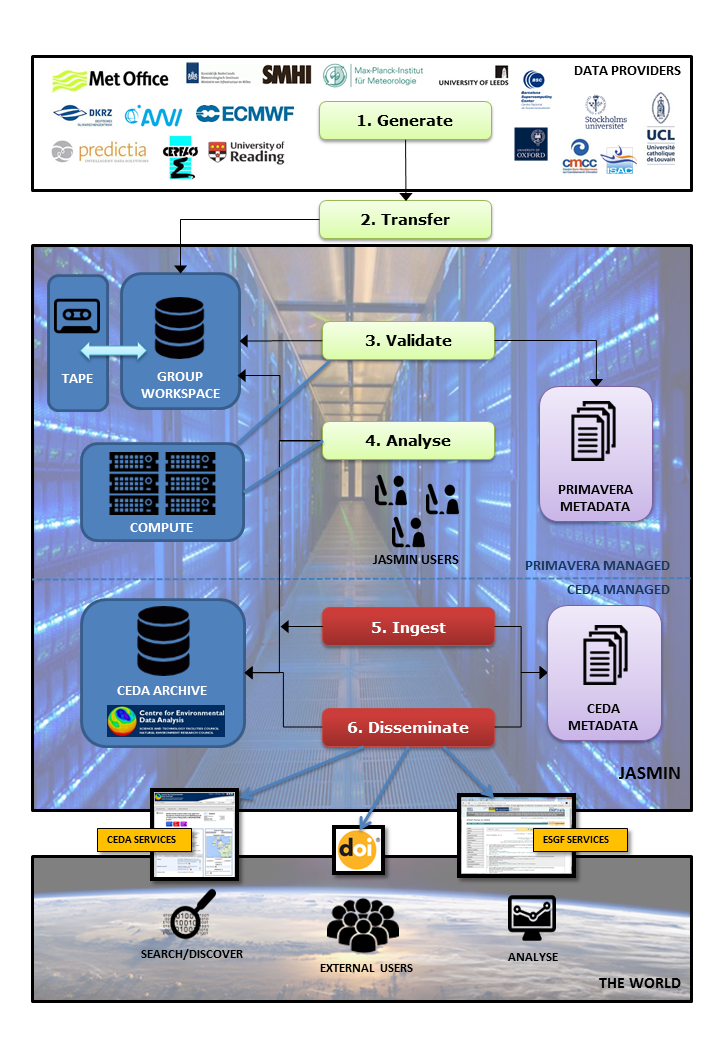
\includegraphics[width=12cm]{original_dmp.png}
\caption{The workflow developed in the Data Management Plan.}
\label{dmp_workflow}
\end{figure*}

Figure~\ref{dmp_workflow} shows the workflow developed in the Data Management Plan (DMP). The workflow can be summarised as taking the analysis to the data. Rather than having copies of the data at users' home institutes, a single copy of the data will be collected at JASMIN. Users are then able to undertake all of the analysis of the data at JASMIN. In the past users have downloaded the files that they want to analyse to computing facilities at their home institute. With the volume of data being produced by PRIMAVERA, it is no longer feasible for everyone to take their own copy of the data.

Step 1 in the DMP workflow is the generation of data  by the modelling centres. The simulations are run at a variety of HPCs across Europe. Each model typically has its own proprietary output file format. Because data was being submitted to HighResMIP the CMIP6 data and metadata standards were chosen for this project~\citep{gmd-11-3659-2018}. These standards include files being saved in netCDF format, the file naming structure and the data request. The HighResMIP data request was developed as part of the CMIP6 data request process. Some additional variables were identified as being required for specific PRIMAVERA analysis bit not being required for HighResMIP. These additional PRIMAVERA specific variables are shown in the PRIMAVERA specific MIP tables~\citep{Nadeau2018}. These PRIMAVERA specific variables will analysed internally to the project at JASMIN and then archived by CEDA separately to the HighResMIP variables. If data has been output by the climate models in a proprietary format then it was post-processed or CMORized (Climate Model Output Rewriter~\cite{Nadeau2019}) into standards compliant files.

The next step in the workflow is the transfer of the data from the HPCs or post-processing systems to JASMIN. A discussion on the transfer techniques used and the rates achieved is given later. The data is uploaded to one of the PRIMAVERA GWS' at JASMIN.

Step 3 in the workflow is the validation of the data. Validation includes checking that the metadata standards have been complied with and the extraction of metadata to store in the PRIMAVERA database~\cite{Seddon2020}. Once the validation is complete then the files are moved from GWS to tape.

After upload and validation of the data, during Step 4 users analyse and work with the uploaded data. The Data Management Tool's (DMT's) web interface allows users to search the database to identify available data. The DMT shows whether files are currently available on disk, or only on tape. If files are only available on tape then users can request that they are restored to tape using the the web interface. The DMT sends an email when their requested data has been restored from tape and is available on GWS. When users have finished working with a dataset then they can mark it as complete using the web interface. If no users are currently using a dataset then it is deleted from GWS to free-up space for other data.

Steps 5 and 6 in the workflow were managed by CEDA rather than the PRIMAVERA project. Uploaded data is ingested into the CEDA archives and can then be disseminated to the global community using CEDA's ESGF node.


\subsection{JASMIN Resources Allocated}

As a result of the DMP, PRIMAVERA was allocated 440~terabytes (TB) of storage split across 5~group workspaces. A server in the JASMIN internal cloud was allocated, which was given a domain name and HTTPS access from outside of JASMIN was granted to it.

It was estimated that around 2~PB of data would be generated by the project. Not all data could therefore be held on disk and the DMT would have to allow data to be efficiently and reliably moved between tape and GWS.

\subsection{Typical Analysis Workflow}

\begin{figure}[t]
	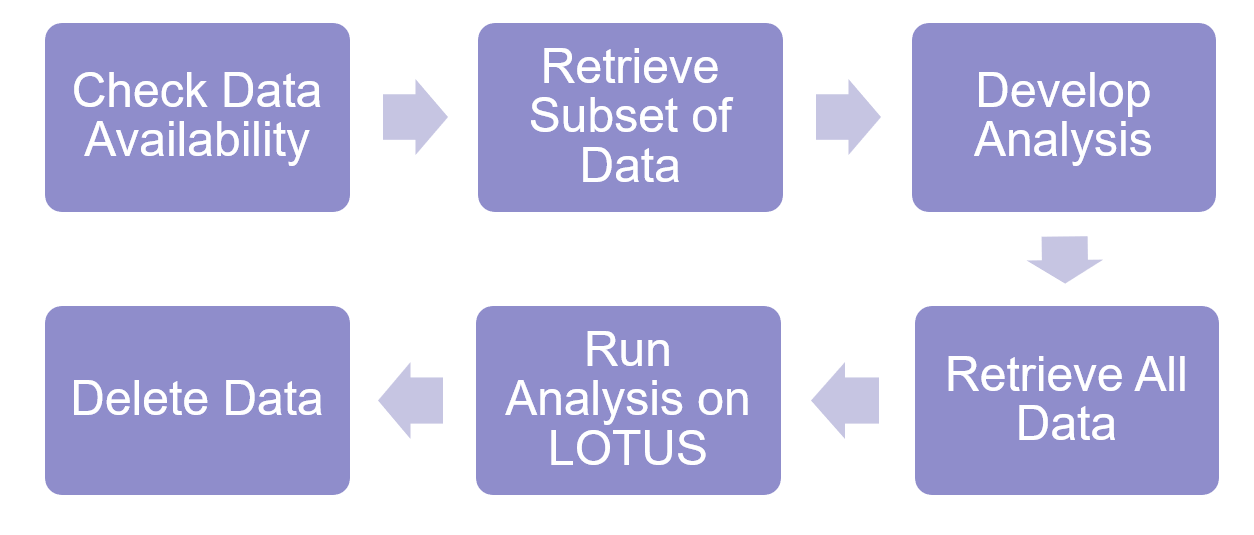
\includegraphics[width=8.3cm]{analysis_workflow.png}
	\caption{The workflow required by users working with the PRIMAVERA data at JASMIN.}
	\label{analysis_workflow}
\end{figure}

Figure~\ref{analysis_workflow} shows the workflow that must be adopted by users working with the PRIMAVERA data at JASMIN. Users would first use th DMT's web interface to identify what data had been uploaded. If they data that they required was not available on disk then they use the DMT's web interface to request that a subset of their data is restored from tape to disk. Once this subset of data is available then they can work on JASMIN's interactive servers to develop and test their analysis code. Once this code has been tested and is working then they use the DMT to request that all of the data that they require is restored from tape to disk. Once the full dataset is available on GWS then the analysis can be run on the LOTUS batch processing cluster. Finally, once users are happy with the results of their analysis then they mark the data as finished in the DMT's web interface. The DMT can then deleted the data from disk to create space for other users' data.

\section{Data Management Tool}

The PRIMAVERA Data Management Tool (DMT) was developed to control the flow of PRIMAVERA data around JASMIN and to allow users to query the available data. The DMT consists of a PostgreSQL database and some custom software written in the Python programming language and uses the Django web framework. The database is installed on the dedicated server, along with a web server and the software. The software was also installed on the JASMIN filesystem and the server's firewall opened to allow database access from JASMIN's interactive servers and from all hosts in the LOTUS cluster. This access allowed the validation of uploaded data to be submitted to the batch processing cluster, where it had access to many nodes, allowing large uploads to be processed in parallel, which is important for processing steps that take a long time, such as calculating checksums.

\begin{figure}[t]
	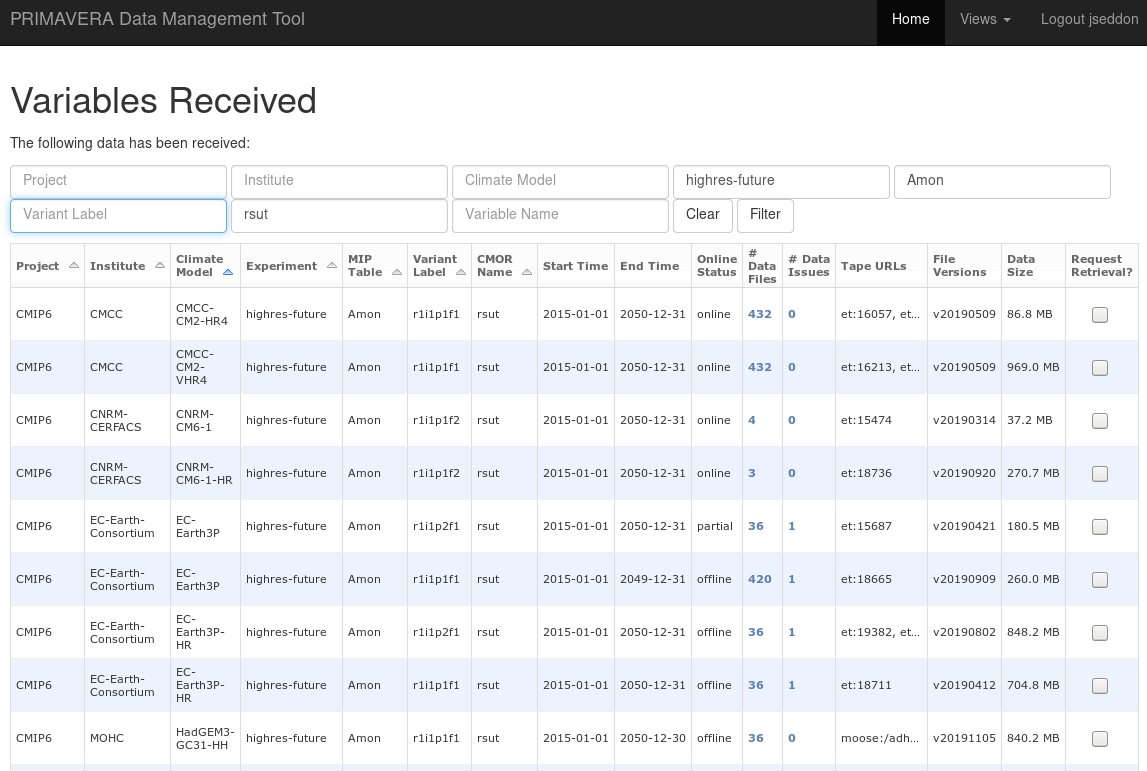
\includegraphics[width=12cm]{dmt_query.png}
	\caption{The workflow required by users working with the PRIMAVERA data at JASMIN.}
	\label{dmt_query}
\end{figure}

A typical screenshot from a user querying the DMT's web interface is shown in Fig.~\ref{dmt_query}. In this example the variable \textit{rsut}, the top of atmosphere outgoing shortwave radiation from the \textit{highres-future}, coupled future experiment is being queried. A value of ``offline'' in the ``Online Status'' column shows that the files for this simulation are currently only available on tape, a value of ``partial'' shows that some files are on disk, but some are only available on tape and ``online'' shows that all files are available on disk. The ``Request Retrieval?'' column allows users to indicate that they want to work with this data. If the data needs to be restored from tape to disk then the user is emailed when the data becomes available. The DMT contains a similar page to allow users to view the data that they've requested and to indicate that it has been finished with and can be deleted from disk if required.

The DMT software is distributed under an open source license~\cite{Seddon2019}. Development of the DMT began in April 2016 and the first data was published in the DMT in May 2017, during this period one developer was largely working full time in its development. Development work has continued intermittently since then to improve the flow of data through the system and to allow the publication of data to the ESGF. 

\section{Data Transfer}

Table~\ref{rates_achieved} shows the sustained rates achieved when transferring data to JASMIN in megabytes per second (MB~s$^{-1}$). JASMIN has several servers in a data transfer zone, whose connection to the Internet and to JASMIN has been designed for maximum throughput in data transfers. At the start of the project it had been assumed that parallel transfer protocols such as BBCP or GridFTP would provide the best transfer rates and data providers were encouraged to use these. In reality, most data providers used the techniques that they were most familiar. The transfer rates achieved depend on many factors including the filesystem at either end, the server and network load at either end and the network between the hosts. The best transfer rate from a site was at least 200~MB~s$^{-1}$, which is 16.5 terabytes per day. 

The transfer of data to JASMIN was only possible because of the transfer rates that could be achieved. Conversely, if JASMIN had not been available to the project then the transfer rates between many different sites would affect the ability to share data.


\section{Future Opportunities}

\subsection{Software}

The DMT software worked well for the PRIMAVERA project but does make some assumptions about the layout of the storage allocated to PRIMAVERA at JASMIN and about the structure of the PRIMAVERA data. The DMT software will require refactoring to generalise it before it can be used in other projects. The current version of the DMT has shown such a tool is feasible and can improve the efficiency of data discovery and storage in such a project.

\subsection{Platforms}

JASMIN has been essential to the success of PRIMAVERA. JASMIN has limited capacity and so may not be able to support all further international projects that would benefit from it. Facilities similar to JASMIN providing additional capacity would be useful for collaborative projects like PRIMAVERA.

Public cloud computing technologies could provide an alternative to a facility such as JASMIN. Users have been using local Unix based computers to analyse data for many years. The change to working remotely at JASMIN was therefore only a small change for them, which was assisted by the existing JASMIN documentation and the development of additional documentation and demonstration videos by the PRIMAVERA project. JASMIN's mix of interactive servers and the batch processing cluster allowed for the easy development of analysis software and then its running on the full multi-model datasets. Moving their analysis to the cloud would be a significant change for users, who would require additional assistance with this. There are however many benefits to the use of public cloud technology such as being able to scale the amount of compute being used to 

Funding for the adoption of public cloud computing would need to be resolved. STFC were PRIMAVERA project partners and received funding for this. Central project funding would be required for the storage of data in the public cloud. Processing in the public cloud is charged per second. It would then have to be decided whether processing would be centrally funded or whether individual institutes or researchers would fund their processing costs. Data sharing outside of the project would be made easier in a public cloud based solution as external users could fund their own processing costs, whereas in PRIMAVERA they have had to be invited onto the JASMIN platform.

New software technologies such as Pangeo offer further benefits if a public cloud solution was used~\citep{Pangeo}. Pangeo is a collection of software packages to enable geoscience research in cloud and HPC environments. It allows data to be distributed across different storage areas and schedules processing on the compute attached to each storage. Pangeo could reduce the volume of data needing to be transferred in future projects. Model output data would be uploaded to a cloud location close to the data provider. Just the metadata would be uploaded to a central (or distributed) catalogue. Tools such as Pangeo would then run users' analysis software on the compute where each dataset is stored and only the small volume of analysis results would need to to transferred.

\conclusions  %% \conclusions[modified heading if necessary]

PRIMAVERA's data management plan and access to the JASMIN super-data-cluster has been essential to the success of the PRIMAVERA project. The DMP and JASMIN have allowed over 100 researchers to collaboratively analyse a multi-model high-resolution set of climate simulations. Over 1.5~PB of data has been collected in a single location where users have been able to analyse the data on interactive data access servers and through a batch processing cluster. The data management tool has reduced the volume of expensive disk storage required by the project by allowing data to be seamlessly moved between tape and disk under the control of data users.

The tools developed by the PRIMAVERA project have successfully demonstrated the feasibility of such techniques. The tools have been made freely available, but as a proof-of-concept, require some development before they can be seamlessly adopted by other projects.

The use of facilities such as JASMIN and the PRIMAVERA DMT have proven successful and are recommended for adoption by other projects. The inclusion in the project proposal of dedicated resource for data management and developing the DMT contributed to the success of the data management.

%% TODO: what didn't work so well???

%% The following commands are for the statements about the availability of data sets and/or software code corresponding to the manuscript.
%% It is strongly recommended to make use of these sections in case data sets and/or software code have been part of your research the article is based on.

\codeavailability{The PRIMAVERA Data Management Tool's source code can be found in a publicly available GitHub repository distributed under a BSD 3-Clause license \citep{Seddon2019}. Additional tools are similarly availble in the validaton tool~\cite{Seddon2020} and MIP tables~\cite{Nadeau2018}.}



% \dataavailability{TEXT} %% use this section when having only data sets available


% \codedataavailability{TEXT} %% use this section when having data sets and software code available


% \sampleavailability{TEXT} %% use this section when having geoscientific samples available


% \videosupplement{TEXT} %% use this section when having video supplements available


%\appendix
%\section{}    %% Appendix A
%
%\subsection{}     %% Appendix A1, A2, etc.


\noappendix       %% use this to mark the end of the appendix section

%% Regarding figures and tables in appendices, the following two options are possible depending on your general handling of figures and tables in the manuscript environment:

%% Option 1: If you sorted all figures and tables into the sections of the text, please also sort the appendix figures and appendix tables into the respective appendix sections.
%% They will be correctly named automatically.

%% Option 2: If you put all figures after the reference list, please insert appendix tables and figures after the normal tables and figures.
%% To rename them correctly to A1, A2, etc., please add the following commands in front of them:

\appendixfigures  %% needs to be added in front of appendix figures

\appendixtables   %% needs to be added in front of appendix tables

\begin{table}[t]
	\caption{The rates achieved while transferring data from the data providers to JASMIN.}
	\begin{tabular}{lll}
		\tophline
		Transfer from & Rate achieved & Protocol used \\
		\middlehline
		Toulouse, France & 13~MB~s$^{-1}$ & 4 BBCP jobs in parallel, with 4 streams each \\
		Hamburg, Germany & 20 to 55~MB~s$^{-1}$ & globus-url-copy \\
		Bologna, Italy & 34~MB~s$^{-1}$ average, 69~MB~s$^{-1}$ peak & gridftp, with 4 concurrent FTP connections 8 process in parallel \\
		Bologna (Cineca), Italy & 200 to 300~MB~s$^{-1}$ & 5 parallel \texttt{rsync -av -e "ssh -c arcfour"} \\
		Barcelona, Spain & 13~MB~s$^{-1}$ & rsync \\
		Exeter, UK & 30~MB~s$^{-1}$ & 5 \texttt{moo get} in parallel \\
		Reading, UK & 85~MB~s$^{-1}$ & 4 parallel \texttt{rsync -rvz --rsh="ssh -c arcfour"} \\
		\bottomhline
	\end{tabular}
	\belowtable{} % Table Footnotes
	\label{rates_achieved}
\end{table}


%% Please add \clearpage between each table and/or figure. Further guidelines on figures and tables can be found below.



\authorcontribution{MM and AS developed the PRIMAVERA data management plan. JS and AS then developed and implemented the DMT and managed the data upload and data availability. JS prepared the manuscript with contributions from all co-authors.} %% this section is mandatory for the journals ACP and GMD. For all other journals it is strongly recommended to make use of this section

\competinginterests{The authors declare that they have no conflict of interest.} %% this section is mandatory even if you declare that no competing interests are present

% \disclaimer{TEXT} %% optional section

\begin{acknowledgements}
The PRIMAVERA project is funded by the European Union's Horizon 2020 programme, Grant Agreement no. 641727. This work used JASMIN, the UK's collaborative data analysis environment (http://jasmin.ac.uk). The authors would like to thank all of the STFC staff who design and maintain JASMIN, without whom this work would not have been possible. The data providers from the PRIMAVERA modelling centres should also be thanked for their hard work complying with the metadata standards and enthusiasm to use the workflows developed in the project.
\end{acknowledgements}




%% REFERENCES

%% The reference list is compiled as follows:

%\begin{thebibliography}{}
%
%\bibitem[AUTHOR(YEAR)]{LABEL1}
%REFERENCE 1
%
%\bibitem[AUTHOR(YEAR)]{LABEL2}
%REFERENCE 2
%
%\end{thebibliography}

%% Since the Copernicus LaTeX package includes the BibTeX style file copernicus.bst,
%% authors experienced with BibTeX only have to include the following two lines:
%%
\bibliographystyle{copernicus}
\bibliography{jasmin-paper.bib}
%%
%% URLs and DOIs can be entered in your BibTeX file as:
%%
%% URL = {http://www.xyz.org/~jones/idx_g.htm}
%% DOI = {10.5194/xyz}


%% LITERATURE CITATIONS
%%
%% command                        & example result
%% \citet{jones90}|               & Jones et al. (1990)
%% \citep{jones90}|               & (Jones et al., 1990)
%% \citep{jones90,jones93}|       & (Jones et al., 1990, 1993)
%% \citep[p.~32]{jones90}|        & (Jones et al., 1990, p.~32)
%% \citep[e.g.,][]{jones90}|      & (e.g., Jones et al., 1990)
%% \citep[e.g.,][p.~32]{jones90}| & (e.g., Jones et al., 1990, p.~32)
%% \citeauthor{jones90}|          & Jones et al.
%% \citeyear{jones90}|            & 1990



%% FIGURES

%% When figures and tables are placed at the end of the MS (article in one-column style), please add \clearpage
%% between bibliography and first table and/or figure as well as between each table and/or figure.


%% ONE-COLUMN FIGURES

%%f
%\begin{figure}[t]
%\includegraphics[width=8.3cm]{FILE NAME}
%\caption{TEXT}
%\end{figure}
%
%%% TWO-COLUMN FIGURES
%
%%f
%\begin{figure*}[t]
%\includegraphics[width=12cm]{FILE NAME}
%\caption{TEXT}
%\end{figure*}
%
%
%%% TABLES
%%%
%%% The different columns must be seperated with a & command and should
%%% end with \\ to identify the column brake.
%
%%% ONE-COLUMN TABLE
%
%%t
%\begin{table}[t]
%\caption{TEXT}
%\begin{tabular}{column = lcr}
%\tophline
%
%\middlehline
%
%\bottomhline
%\end{tabular}
%\belowtable{} % Table Footnotes
%\end{table}
%
%%% TWO-COLUMN TABLE
%
%%t
%\begin{table*}[t]
%\caption{TEXT}
%\begin{tabular}{column = lcr}
%\tophline
%
%\middlehline
%
%\bottomhline
%\end{tabular}
%\belowtable{} % Table Footnotes
%\end{table*}
%
%%% LANDSCAPE TABLE
%
%%t
%\begin{sidewaystable*}[t]
%\caption{TEXT}
%\begin{tabular}{column = lcr}
%\tophline
%
%\middlehline
%
%\bottomhline
%\end{tabular}
%\belowtable{} % Table Footnotes
%\end{sidewaystable*}
%
%
%%% MATHEMATICAL EXPRESSIONS
%
%%% All papers typeset by Copernicus Publications follow the math typesetting regulations
%%% given by the IUPAC Green Book (IUPAC: Quantities, Units and Symbols in Physical Chemistry,
%%% 2nd Edn., Blackwell Science, available at: http://old.iupac.org/publications/books/gbook/green_book_2ed.pdf, 1993).
%%%
%%% Physical quantities/variables are typeset in italic font (t for time, T for Temperature)
%%% Indices which are not defined are typeset in italic font (x, y, z, a, b, c)
%%% Items/objects which are defined are typeset in roman font (Car A, Car B)
%%% Descriptions/specifications which are defined by itself are typeset in roman font (abs, rel, ref, tot, net, ice)
%%% Abbreviations from 2 letters are typeset in roman font (RH, LAI)
%%% Vectors are identified in bold italic font using \vec{x}
%%% Matrices are identified in bold roman font
%%% Multiplication signs are typeset using the LaTeX commands \times (for vector products, grids, and exponential notations) or \cdot
%%% The character * should not be applied as mutliplication sign
%
%
%%% EQUATIONS
%
%%% Single-row equation
%
%\begin{equation}
%
%\end{equation}
%
%%% Multiline equation
%
%\begin{align}
%& 3 + 5 = 8\\
%& 3 + 5 = 8\\
%& 3 + 5 = 8
%\end{align}
%
%
%%% MATRICES
%
%\begin{matrix}
%x & y & z\\
%x & y & z\\
%x & y & z\\
%\end{matrix}
%
%
%%% ALGORITHM
%
%\begin{algorithm}
%\caption{...}
%\label{a1}
%\begin{algorithmic}
%...
%\end{algorithmic}
%\end{algorithm}
%
%
%%% CHEMICAL FORMULAS AND REACTIONS
%
%%% For formulas embedded in the text, please use \chem{}
%
%%% The reaction environment creates labels including the letter R, i.e. (R1), (R2), etc.
%
%\begin{reaction}
%%% \rightarrow should be used for normal (one-way) chemical reactions
%%% \rightleftharpoons should be used for equilibria
%%% \leftrightarrow should be used for resonance structures
%\end{reaction}
%
%
%%% PHYSICAL UNITS
%%%
%%% Please use \unit{} and apply the exponential notation


\end{document}
